\documentclass[11pt]{article}
\usepackage[margin=2.2cm]{geometry}
\usepackage{booktabs}
\usepackage{float}
\usepackage{graphicx}
\title{TF-Number Experiment 2}
\author{}
\date{}
\begin{document}
\maketitle
This experiment holds the input at 3,000 highly variable genes and varies the requested TF count.
The bipartite-retained count is measured by \texttt{limit-tfs.py}; the causal-graph count is measured after top-15 TF subsetting by \texttt{grn\_creation.py}.
\begin{equation}
\widehat{M}(x) = -4.9099x + 16093.5\ \mathrm{MiB},\qquad R^2=0.9954
\end{equation}
\begin{equation}
\widehat{t}(x) = -0.06489x + 239.09\ \mathrm{ms/step},\qquad R^2=0.9761
\end{equation}
The fits are ordinary least-squares fits over the completed runs and use requested TFs as $x$.
\subsection{Requested TFs versus Target Genes}
Target-gene count is not a better predictor in this experiment: its linear fits have $R^2=0.9954$ for memory and $R^2=0.9761$ for time, identical to the requested-TF fits. This is expected because the runs use a fixed 3,000-gene input and satisfy $\mathrm{targets}=3{,}000-\mathrm{requested\ TFs}$ (apart from graph genes excluded for lack of regulators).
The equivalent target-based fits are:
\begin{equation}
\widehat{M}(y) = 4.9099y + 1363.9\ \mathrm{MiB},\qquad R^2=0.9954
\end{equation}
\begin{equation}
\widehat{t}(y) = 0.06489y + 44.43\ \mathrm{ms/step},\qquad R^2=0.9761
\end{equation}
\begin{table}[H]
\centering
\small
\caption{Requested and effective TF counts, plus final causal-graph size.}
\begin{tabular}{rrrrrrrr}
\toprule
Requested & Bipartite retained & Graph TFs & Targets & Genes & Possible edges & Imposed edges & Density\\
\midrule
100 & 100 & 100 & 2,900 & 3,000 & 290,000 & 41,557 & 14.3\%\\
200 & 200 & 200 & 2,800 & 3,000 & 560,000 & 41,610 & 7.4\%\\
300 & 300 & 300 & 2,700 & 3,000 & 810,000 & 40,362 & 5.0\%\\
400 & 400 & 400 & 2,600 & 3,000 & 1,040,000 & 38,934 & 3.7\%\\
500 & 500 & 500 & 2,500 & 3,000 & 1,250,000 & 37,469 & 3.0\%\\
600 & 600 & 600 & 2,400 & 3,000 & 1,440,000 & 35,986 & 2.5\%\\
700 & 700 & 700 & 2,300 & 3,000 & 1,610,000 & 34,499 & 2.1\%\\
800 & 800 & 800 & 2,200 & 3,000 & 1,760,000 & 33,000 & 1.9\%\\
900 & 900 & 900 & 2,100 & 3,000 & 1,890,000 & 31,500 & 1.7\%\\
1,000 & 1,000 & 1,000 & 2,000 & 3,000 & 2,000,000 & 30,000 & 1.5\%\\
1,100 & 1,100 & 1,100 & 1,900 & 3,000 & 2,090,000 & 28,500 & 1.4\%\\
1,200 & 1,200 & 1,200 & 1,800 & 3,000 & 2,160,000 & 27,000 & 1.2\%\\
1,300 & 1,300 & 1,300 & 1,700 & 3,000 & 2,210,000 & 25,500 & 1.2\%\\
1,400 & 1,400 & 1,399 & 1,600 & 2,999 & 2,238,400 & 24,000 & 1.1\%\\
1,500 & 1,500 & 1,496 & 1,500 & 2,996 & 2,244,000 & 22,500 & 1.0\%\\
1,600 & 1,600 & 1,586 & 1,400 & 2,986 & 2,220,400 & 21,000 & 0.9\%\\
1,700 & 1,699 & 1,668 & 1,300 & 2,968 & 2,168,400 & 19,500 & 0.9\%\\
1,800 & 1,798 & 1,739 & 1,200 & 2,939 & 2,086,800 & 18,000 & 0.9\%\\
1,900 & 1,894 & 1,803 & 1,100 & 2,903 & 1,983,300 & 16,500 & 0.8\%\\
2,000 & 1,988 & 1,844 & 1,000 & 2,844 & 1,844,000 & 15,000 & 0.8\%\\
2,100 & 2,076 & 1,872 & 900 & 2,772 & 1,684,800 & 13,500 & 0.8\%\\
2,200 & 2,163 & 1,873 & 800 & 2,673 & 1,498,400 & 12,000 & 0.8\%\\
2,300 & 2,244 & 1,834 & 700 & 2,534 & 1,283,800 & 10,500 & 0.8\%\\
2,400 & 2,311 & 1,782 & 600 & 2,382 & 1,069,200 & 9,000 & 0.8\%\\
2,500 & 2,354 & 1,699 & 500 & 2,199 & 849,500 & 7,500 & 0.9\%\\
2,600 & 2,351 & 1,577 & 400 & 1,977 & 630,800 & 6,000 & 1.0\%\\
2,700 & 2,318 & 1,406 & 300 & 1,706 & 421,800 & 4,500 & 1.1\%\\
2,800 & 2,178 & 1,155 & 200 & 1,355 & 231,000 & 3,000 & 1.3\%\\
2,900 & 1,853 & 792 & 100 & 892 & 79,200 & 1,500 & 1.9\%\\
\bottomrule
\end{tabular}
\end{table}
\begin{table}[H]
\centering
\small
\caption{Measured causal-generator time and memory requirements.}
\begin{tabular}{rrrr}
\toprule
Requested TFs & Target genes & Avg step time (ms) & Peak memory (MiB)\\
\midrule
100 & 2,900 & 226 & 14,545\\
200 & 2,800 & 236 & 14,843\\
300 & 2,700 & 217 & 14,829\\
400 & 2,600 & 211 & 14,365\\
500 & 2,500 & 219 & 13,541\\
600 & 2,400 & 212 & 13,049\\
700 & 2,300 & 192 & 13,059\\
800 & 2,200 & 184 & 12,393\\
900 & 2,100 & 178 & 11,881\\
1,000 & 2,000 & 157 & 11,125\\
1,100 & 1,900 & 164 & 11,041\\
1,200 & 1,800 & 173 & 10,371\\
1,300 & 1,700 & 150 & 9,869\\
1,400 & 1,600 & 149 & 9,029\\
1,500 & 1,500 & 151 & 8,863\\
1,600 & 1,400 & 131 & 8,373\\
1,700 & 1,300 & 134 & 7,865\\
1,800 & 1,200 & 107 & 7,365\\
1,900 & 1,100 & 116 & 6,857\\
2,000 & 1,000 & 114 & 6,371\\
2,100 & 900 & 109 & 5,869\\
2,200 & 800 & 81 & 5,043\\
2,300 & 700 & 78 & 4,465\\
2,400 & 600 & 88 & 4,295\\
2,500 & 500 & 67 & 3,787\\
2,600 & 400 & 72 & 3,419\\
2,700 & 300 & 65 & 2,885\\
2,800 & 200 & 69 & 1,899\\
2,900 & 100 & 61 & 1,837\\
\bottomrule
\end{tabular}
\end{table}
\begin{figure}[H]\centering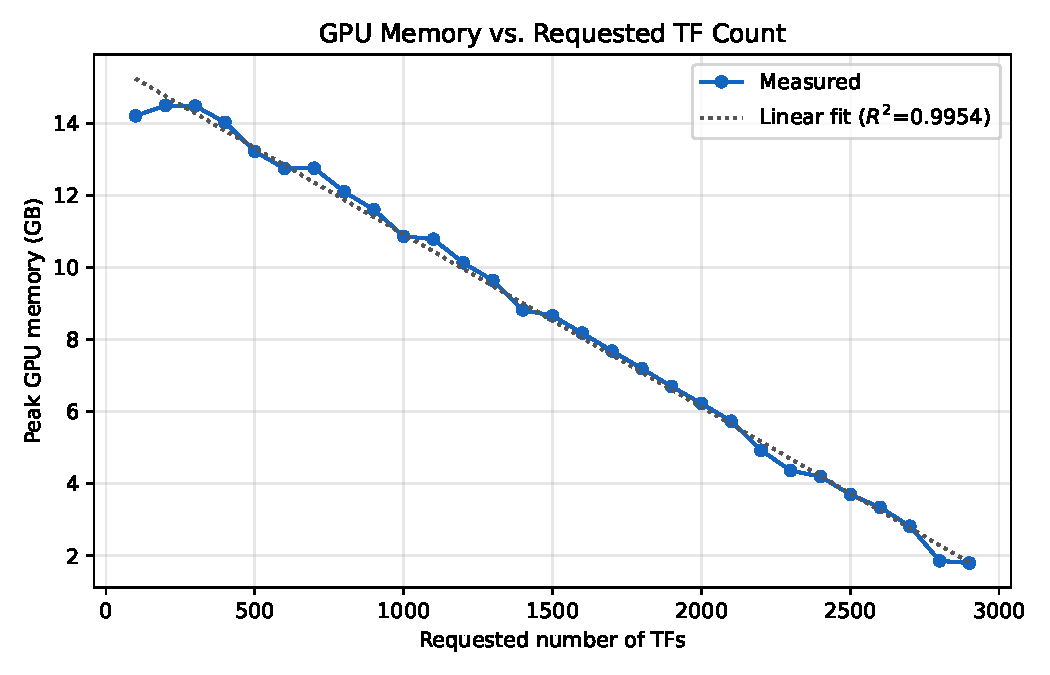
\includegraphics[width=0.9\textwidth]{memory_vs_requested_tfs.pdf}
\caption{Peak GPU memory requirement versus requested TF count.}\end{figure}
\begin{figure}[H]\centering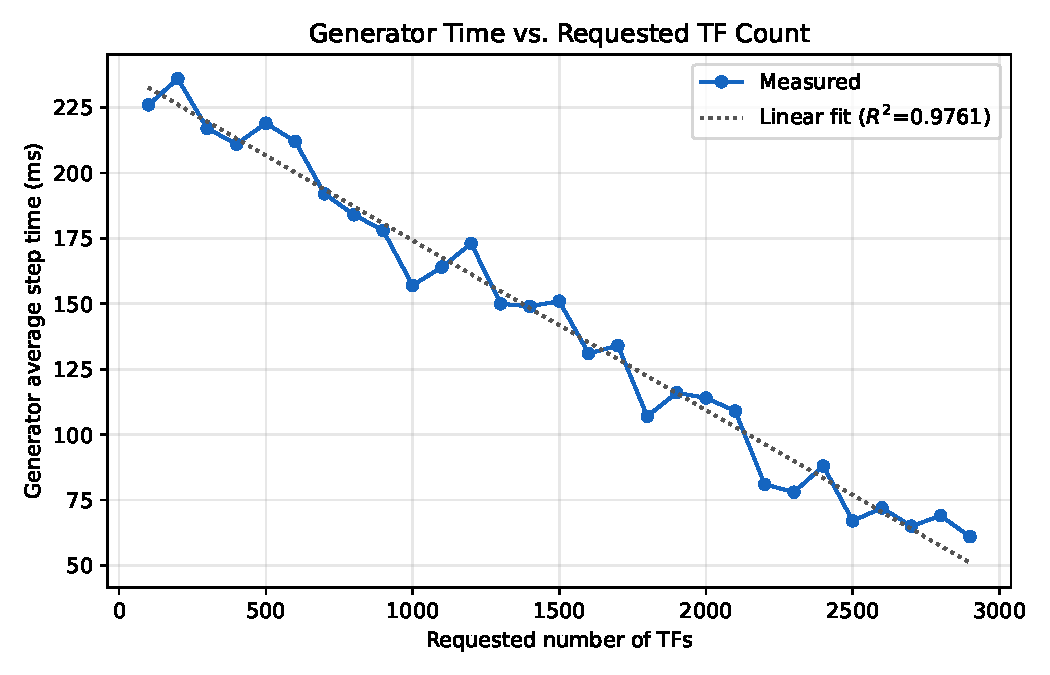
\includegraphics[width=0.9\textwidth]{time_vs_requested_tfs.pdf}
\caption{Causal-generator average step time versus requested TF count.}\end{figure}
\end{document}
